% Summary of baker2013: Agreement and case

\begin{abstract}
Summarizes the history of case and agreements theories, the main empirical facts motivating each theory, and the parallelisms between case, agreement, and concord.

Spec-Head Agreement was motivated by the fact that Tense seemed to agree with whatever was put in specTP. Probe-Goal Agreement was motivated empirically by Expletive Constructions, Ergativity, and Long-Distance Agreement.

Agreement and Concord are probably the same thing, but then Upwards Agree becomes much more necessary. Dependent case explains a lot, but potentially weakens the link between case and agreement. Agreement between a subject and a predicate nominal is probably semantic.

\textit{This part is mostly my interpretation, not explicitly discussed:}

Spec-Head and Probe-Goal are causally inverses:

\begin{itemize}
  \item the former treats movement as a near-prerequisite for agreement, and the latter treats agreement as a prerequisite for movement.
\end{itemize}
For the most part, they have similar locality conditions:

\begin{itemize}
  \item look down, relativized minimality, phasehood
\end{itemize}
But they each make one special prediction:

\begin{itemize}
  \item Spec-Head predicts heads can agree with XPs generated in their specifiers
  \item Probe-Goal predicts heads can agree with XPs that don't reach their specifiers
\end{itemize}

Key empirical facts to explain:

\begin{enumerate}
  \item Subject-Verb agreement on T
  \item French and Italian participial agreement with raised objects
  \item Bantu T agreement with fronted locatives and objects
  \item Arabic more agreement in SVO than VSO
  \item English T still agrees with unraised subjects in expletive constructions and locative inversion
  \item Hindi perfective verbs agree with bare NP objects (the first nominatives)
  \item Tsez verbs agree with embedded topicalized arguments
  \item Kiswahili verbs object-agree with goals if they exist, otherwise themes
  \item Kiswahili object agreement is impossible in passive clauses
  \item Welsh prepositions agree with their complements
  \item West Flemish complementizers agree with their embedded subjects (along with T which also agrees)
  \item Zulu verbs agree with their highest object but only if that object is definite
  \item Amharic subject agreement doesn't require definiteness, but object agreement does
  \item Nahuatl allows object agreement with indefinite objects inside the VP
  \item Lubukusu complementizers agree with the subject of the matrix clause
  \item Adjectives don't agree in person
  \item Multiple adjectives agree with the same noun
  \item Burushaski verbs agree with the thematic subject and object, not changing agreement patterns when they get different cases (nominative, accusative, dative, ergative).
\end{enumerate}
\end{abstract}

\section*{Introduction}

Core cases of Agreement:

\begin{itemize}
  \item morphological marking on the central verb of a clause, reflecting some features of an NP in the clause.
\end{itemize}

Extensions from this core:

\begin{itemize}
  \item Verb agreeing with the features of an NP that is not the subject
  \item Non-verb agreeing with a nearby NP (possessed noun with possessor, or preposition with complement)
\end{itemize}

Maybe agreement:

\begin{itemize}
  \item Adjectives, determiners, `modifiers' agreeing with their head noun (Concord)
  \item Something agreeing with non-NP things (Serial Verb Constructions, NPs matching the tense of the verb like in Kayardild Evans 1995)
  \begin{itemize}
    \item exclude these because very little discussed, but interesting
  \end{itemize}
\end{itemize}

Core cases of Case:

\begin{itemize}
  \item morphological marking on an NP reflecting some aspect of its grammatical relationship to a central verb of the clause (nominative, accusative, dative)
\end{itemize}

Extensions from this core:

\begin{itemize}
  \item NPs related to other kinds of categories (genitive)
  \item non-NPs (e.g. embedded, non-finite verbs)
\end{itemize}

$\rightarrow$ Agreement and Case are kind of opposites.

\begin{itemize}
  \item Head-marking languages are roughly languages rich in agreement
  \item Dependent-marking languages are roughly languages rich in case
  \item both are extremely common but not universal
\end{itemize}

Some generative linguists think they're manifestations of the same abstract relationship (Chomsky 2000, Chomsky 2001, origins of this view in George and Kornfilt 1981)

\begin{itemize}
  \item in many Indo-European languages, a verb agrees with an NP iff it bears [nom].
  \item Chomsky 2000, 2001 posited Agree as one of only two primitive syntactic operations
\end{itemize}

\section*{Syntax of Agreement}

Most accounts start with Subject-Verb Agreement:

\begin{itemize}
  \item most common (found in around 75\% of languages, whereas object agreement is found in around 50\%)
  \item typological near-universal: languages never agree with direct objects without agreeing with some subjects too
  \item subject agreement is the only kind found in the most accessible and well-studied languages (e.g. IE)
\end{itemize}

In IE languages, agreement only shows up on tensed verbs - why?

\begin{itemize}
  \item Because T and V are separate, and it is T that agrees with the NP.
\end{itemize}

The verb also agrees with the subject - why?

\begin{enumerate}
  \item If agreement takes place after movement, then T needs to look towards specTP: the Spec-Head Agreement hypothesis.
  \item If agreement takes place before movement, then T needs to `probe down', and the subject is the first thing it sees: the Probe-Goal Agreement hypothesis.
\end{enumerate}
\#me Both hypotheses have essentially the same motivation (the subject is the highest NP, whether it is found by Agree or Move first), but different restrictions on when agreement must take place.

\subsection*{Motivation for Spec-Head Agreement}

Dominated generative research from about 1985-1999, since Chomsky 1986 regularized the role of Tense within the X-bar system.

Popularity fueled by Kayne 1989 on French and Italian agreement.

\begin{itemize}
  \item Kayne: the verb does agree with the DO, but only when the verb is a participial, and the DO moves higher than it (Wh-movement or Passivization), and uses specTP as a landing point (for him, specPtpl)
\end{itemize}

Also fueled by studies on Bantu languages like Kiswahili and Kilega in e.g. Kinyalolo 1991.

\begin{itemize}
  \item In Kilega, when a locative moves to specTP (Locative Inversion), T agrees with the locative and not the subject.
  \item In some other Bantu languages, this happens with the fronted object.
\end{itemize}

Another fairly simple example was in Classical Arabic.

\begin{itemize}
  \item Verbs shows full agreement in SVO order, with the subject arguably moving to specTP, but reduced agreement in VSO order, when the subject doesn't move to specTP (Koopman and Sportiche 1991, Fassi Fehri 1993)
\end{itemize}

\subsection*{Motivation for Probe-Goal Agreement}

Partly motivated by abstract considerations of Minimalism.

\begin{itemize}
  \item Wanted to replace Move as a primitive syntactic operation, to explain why it seems to function as a last resort, pre-empted by other operations.
  \item Therefore identified Merge and Agree as the fundamental ones.
\end{itemize}

He made X agreeing with Y a \textit{precondition} for Y moving to specX, rather than a \textit{result} of it.

\#me So really, Spec-Head vs. Probe-Goal is a question of timing.

Empirically, it also helped with some facts:

\begin{itemize}
  \item English Expletive Constructions have specTP empty with a placeholder, but tense can still agree with the subject, which is lower.
  \item English does have locative inversion, but the verb agrees with the subject still (``Mary said that on the table were put peanuts.'')
  \item Hindi-Urdu perfective verbs agree with bare NP objects (rather than ergative subjects) - they probably don't move to specTP
\end{itemize}

Other ways to interpret these facts, taken by Koopman 2005 to go back to Spec-Head, or by Franck et al. 2006 to add it alongside Probe-Goal

\begin{itemize}
  \item The English locative moves overtly to specTP and then is reconstructed back in its original position, \textit{or} it moves to a clause-initial position other than specTP
  \item The Hindi object is in specTP at one point in the derivation, before further movements separate them again.
\end{itemize}

However, Probe-Goal has become the dominant hypothesis.

\subsection*{Preconditions on Probe-Goal Agree}

\begin{enumerate}
  \item The agreeing head must search downward, not upward or sideward.
  \item The Intervention Condition: the agreeing head must agree with the closest element it finds with the relevant features.
  \item The Activity Condition: in order for an NP to be eligible for agreement, it must have an unvalued uninterpretable feature. \textbf{In practice, this is a case feature, since features like number, gender, and person are interpretable.}
  \begin{itemize}
    \item Practical effect: T can't agree with an NP that has already received case from some other source.
    \begin{itemize}
      \item T can't agree with Icelandic subjects that have already received idiosyncratic dative case from lexical verbs/adjectives.
      \item T can't agree with objects of English prepositional phrases (``it seem*(s) to some linguists that agreement is a fascinating topic'')
    \end{itemize}
  \end{itemize}
  \item The Phase Condition, a result of the more general Phase Impenetrability Condition, that things can't agree with things in lower phases.
  \begin{itemize}
    \item T doesn't agree with the subjects of embedded clauses.
  \end{itemize}
\end{enumerate}

Turns out that Long-Distance Agreement does exist though:

\begin{itemize}
  \item Some languages permit a functional head in the matrix clause to agree with an NP in an embedded clause (Tsez, verb, Polinsky and Potsdam 2001)
\end{itemize}

Most literature thinks the Phase Condition still holds, and explains subtleties with LDA:

\begin{itemize}
  \item In Tsez, LDA is only possible if the embedded NP is topicalized - at specCP and accessible to higher phases.
  \item Similar accounts for Algonquian languages like Passamaquoddy and Innu-Aimun (Bruening 2001, Branigan and MacKenzie 2002)
\end{itemize}

Also other kinds of LDA, like `restructuring' cases where the embedded clause is really only a VP, not a phase.

Polinsky 2003 is a good overview of various analytical options available for explaining different kinds of LDA.

Also Frank 2006 and Etxepare 2006 on the possibility of indirect local agreement.

\#me what is indirect local agreement?

\subsection*{Object Agreement}

Ideas about the relationship between case and agreement imply that object agreement happens even in English, because agreement is how objects get accusative case.

Widely assumed: some functional head between little-v and big-V agrees with objects.

\begin{itemize}
  \item predicts object agreement agrees with the highest object (the goal in constructions with both a theme and a goal) (Boeckx and Niinuma 2004)
  \begin{itemize}
    \item pans out in a lot of languages, including Kiswahili
  \end{itemize}
\end{itemize}

Which FP agrees with objects?

\begin{enumerate}
  \item Inner aspect head (Travis 1991)
  \item Dedicated agreement head with no semantic content (Chomsky 1991, Koizumi 1995)
  \item Most widely held view: the transitive little-v itself (the same head that semantically regulates the subject)
  \begin{itemize}
    \item Backed up by the fact that object agreement is impossible in passive clauses in many languages (even when the verb is ditransitive so there's still an object to agree with)
  \end{itemize}
\end{enumerate}

\subsection*{Agreement on Adpositions}

Found in 20-30\% of languages, depending on which are analyzed as clitics.

\begin{itemize}
  \item Welsh prepositions agree with pronominal objects ``about-3sg him''
\end{itemize}

Supports Probe-Goal over Spec-Head.

\subsection*{Agreement on Complementizers}

Not very common.

\begin{itemize}
  \item Dutch and German C agrees with the subject of its TP complement
\end{itemize}

Also supports Probe-Goal over Spec-Head.

However, in these cases T also agrees with the subject first, which should make it hard for C to agree due to the Activity Condition.

\begin{itemize}
  \item Answer: C and T are closely related, so may not count as different heads for purposes of case and agreement (Chomsky 2008, T inherits agreement features from C, discussion in Carstens 2003, van Koppen 2005)
\end{itemize}
\#me very interesting

\subsection*{Object Agreement: Sensitivity to Specificity}

One might think that object agreement supports Probe-Goal over Spec-Head, since objects are lower than little-v.

However, unlike other types of agreement, object agreement is often related to the specificity of the agreed-with nominal.

\begin{itemize}
  \item Zulu verbs agree with their highest object only if that object is specific
  \begin{itemize}
    \item e.g. definite
  \end{itemize}
  \item In Amharic, subjects of all kinds trigger agreement, but only specific objects trigger agreement
\end{itemize}

In the Syntax-semantics Interface literature, some people think that (only) objects that have been moved away from the verb are specific (Diesing 1992).

However, this can also be explained by Probe-Goal in that only when the object moves out of the VP phase can it agree with vP.

\subsection*{Object Agreement vs Pronominal Cliticization}

Hard to tease apart empirically:

\begin{itemize}
  \item I really like-3sg that girl.
  \item That girl, I really like her.
\end{itemize}

Big debate in language families like Romance, Bantu, Hungarian, Amharic, etc.

This analytical ambiguity is presumably a source of language change, with cliticization leading to agreement.

Similar issues arise distinguishing subject agreement and subject clitics (e.g. Culbertson 2010 on French).

\subsection*{Parameters of Agreement}

What heads participate:

\begin{itemize}
  \item T agrees in English and Kinande, but not Japanese
  \item transitive little-v ageres in Kiswahili, but not English
  \item P agrees in Welsh, but not English
  \item C agrees in West Flemish, but not standard Dutch
\end{itemize}

This is just variation in the lexicon, what you'd expect in Minimalism.

However, there are also other more subtle parameters.

\begin{itemize}
  \item Nahuatl and some other languages allow object agreement with an indefinite object inside the VP.
\end{itemize}

Maybe Spec-Head is true for Bantu, and Probe-Goal is true for IE. Two ways of stating such a parameter:

\begin{itemize}
  \item Carstens 2005: Probe-Goal, but Bantu languages are also subject to another principle:
  \begin{itemize}
    \item if F agrees with X, then X must check an EPP feature of F (= if agree, then must move to spec)
  \end{itemize}
  \item Baker 2008: more radical: both Upwards Agree and Downwards Agree exist; Bantu has the former
\end{itemize}

Baker's proposal would explain Resumption in Bantu PPs, where the P agrees with its object only if that object has moved out.

This would also explain why some Bantu Cs agree with the subject of the higher matrix clause.

\begin{itemize}
  \item Diercks 2010: this is really agreement with a Null Operator in SpecCP controlled by the matrix subject
  \begin{itemize}
    \item Similar to many accounts of Logophoric Pronouns in African languages
  \end{itemize}
\end{itemize}

\begin{center}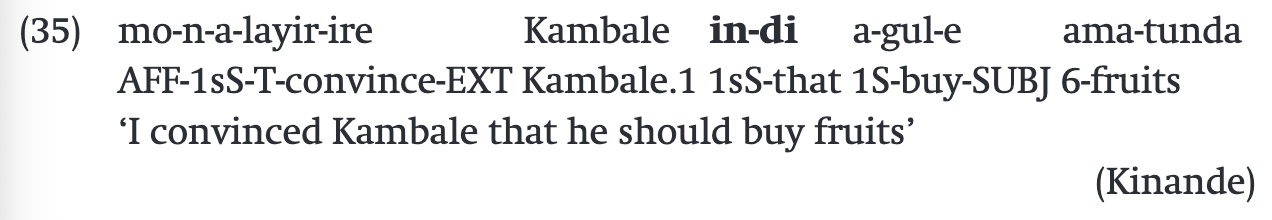
\includegraphics[width=0.72\linewidth]{images/pasted-20260921070718.png}\end{center}

\subsection*{Concord}

Different morphemes than verbal agreement.

Sometimes also different features:

\begin{itemize}
  \item Adjectives don't agree in person. \#me is this a universal?
\end{itemize}

Different restrictions:

\begin{itemize}
  \item Multiple adjectives agree with a single noun, but two verbs (in English at least) don't agree with the same subject.
\end{itemize}

But also some similarities:

\begin{itemize}
  \item ``there are likely to be'` and ``there seems to be'', in languages where adjectives agree (e.g. Icelandic, show the exact same properties and what they agree with
\end{itemize}

Baker 2008 argues they are the same because of this, and says Agree needs two tweaks:

\begin{enumerate}
  \item Can be upwards in addition to downwards:
  \begin{enumerate}
    \item F agrees with XP only iff F c-commands XP or XP c-commands F
  \end{enumerate}
  \item Activity condition goes both ways:
  \begin{enumerate}
    \item F agrees with NP X only if F determines the case feature of NP (case assignment) or NP determines the case feature of F (case concord)
  \end{enumerate}
\end{enumerate}
\#me both of Baker's tweaks are essentially just making Agree truly reciprocal

\#me doesn't say anything about why case concord happens though; kind of shifts the problem - Baker discusses this soon after.

The last case is subject-predicate agreement in predicate nominal sentences, but Baker thinks this is semantic, and it often can be gotten around via semantics (``these clouds are a sign of rain'').

\section*{Case Assignment}

Throughout the 1980s, following Chomsky 1981, case assignment and the Case Filter (all NPs must be assigned case) were super important.

\begin{itemize}
  \item It forced NPs to move, determined stuff like PRO and expletives
\end{itemize}

But Chomsky's promotion of Agree relegated case (plus some debates about how adequate the 80s explanations were)

In the Government and Binding Era, the precondition for case assignment was Government (mutual c-command).

\begin{itemize}
  \item But then definitions of government became more and more complicated in order to allow T to assign nominative case to specTP, and \textit{expect} to assign accusative case to the subject of its nonfinite complement, leading Chomsky to abandon government in the Minimalist Program
\end{itemize}

Chomsky 2000, 2001: case is just Agree.

\begin{itemize}
  \item explains most basic stuff, including ECM
\end{itemize}

However, in order to explain why the subject of ``the ship sank'' doesn't get accusative, Chomsky and others assume there is no little-v there, or perhaps a different sort of little-v which doesn't assign accusative (Burzio's Generalization, Burzio 1986).

\begin{itemize}
  \item no different than saying finite T does agreement, but non-finite T doesn't.
  \item but more deeply, this seems like just a stipulation. Agree has a way to \textit{encode} Burzio's, but not \textit{explain} it.
\end{itemize}

Pretty simple to get genitive (by D) and prepositional (by various Ps) case assignment with Agree.

\subsection*{Prepositional-like cases without prepositions (Semantic case)}

E.g. dative for goals of motion, ablative for sources of motion, instrumental, etc.

More in-line with thematic roles, and these cases don't tend to appear or disappear from NPs depending on structural factor.

Treated differently in virtually every developed case theory.

Often analyzed essentially as Ps.

Three ways to analyze this:

\begin{enumerate}
  \item P is phonologically null but assigns a special case like dative or ablative to its NP complement (Emonds 1985, McFadden 2004)
  \begin{itemize}
    \item most likely analysis for many Germanic and Slavic languages
  \end{itemize}
  \item P is overt, assigns phonologically null case to NP, and fuses with the NP at PF
  \begin{itemize}
    \item most likely for Hungarian (den Dikken 2005, s4.2.3)
  \end{itemize}
  \item Both elements could be spelled out overtly
  \begin{itemize}
    \item source of bimorphemic/trimorphemic cases found in languages with big case systems like Finnish, Estonian, and Lezgian
  \end{itemize}
\end{enumerate}

The boundary between these and normal cases isn't always clear, especially with dative, genitive, and sometimes instrumental.

\subsection*{Lexical case}

Dative subjects in Icelandic.

\begin{itemize}
  \item tend to be experiencers
  \item but idiosyncratic variation and not hard and fast
\end{itemize}

\subsection*{Ergativity and parameters of case assignment}

Ergativity:

\begin{itemize}
  \item subject of transitive clause bears a distinctive case, while subject of intransitive and object of transitive bear the same case
\end{itemize}

Generally, word order, binding, control, and other syntactic relations are what one would expect in nominative-accusative languages.

Views have changed a lot with each framework.

Most widespread view at present:

\begin{itemize}
  \item ergative case is semantic case or lexical case assigned by transitive little-v to its subject in specvP (e.g. Woolford 2006)
\end{itemize}

But then not clear why it varies with aspect.

In Burushaski T agrees with the thematic subject regardless of whether it has ergative or nominative/absolutive case, and transitive little-v agrees with some absolutive arguments (thematically the direct objects but not agentive intransitive subjects) (Baker 2008).

Thus Baker claims there's a second major parameter:

\begin{enumerate}
  \item F agrees with DP/NP only if F values the case feature of DP/NP or vice versa.
\end{enumerate}

\subsection*{Dependent case (and more ergativity)}

Marantz 1991, this formulation from Baker and Vinokurova 2010:

\begin{enumerate}
  \item if there are two distinct argumental NPs in the same phase such that NP1 c-commands NP2, then value the case feature of NP2 as accusative (unless NP1 has already been marked for case)
  \item if there are two distinct NPs in the same phase such that NP1 c-commands NP2, then value the case feature of NP1 as ergative
  \item otherwise, mark NP as nominative/absolutive
\end{enumerate}

Ergative languages are therefore just those that mark the higher of the two NPs in a phase rather than the lower one.

Also extends nicely to tripartite systems like Nez Perce.

\subsection*{Differential Argument Marking}

Differential object marking survey: Aissen 2003.

Dependent case helps with this, because if specific/definite objects move out of the VP phase into the CP phase, then they become the lower of two NPs and get accusative, whereas if they stay in the VP phase, they don't need that.

Also makes sense then that in Nez Perce when the same thing happens (definite objects shift and receive accusative), the subject gets ergative, but with indefinite arguments that don't get accusative, the subject gets nominative.
